\chapter{Vyhodnotenie získaných výsledkov}\label{chap:results}

\section{Detekcia}

Postupne sme natrénovali tri modely, každý s inou verziou dát. Všetky modely mali pre tréning rovnako nastavené parametre, líšili sa jedine verziou dát. Počet epoch bol nastavený na 128, veľkosť dávky na 16 a ostatné boli ponechané s prednastavenými hodnotami. Najlepšie počiatočné váhy, s ktorými dokázal server pracovať mali označenie YOLOv8large.
\\
\begin{table}[ht]
\centering
\begin{tabular}{ |c c c c c|  }
\hline
model  &  presnosť & citlivosť & mAP50 & mAP50-95 \\
\hline
M1  & 0.473 & 0.352	& 0.327	& 0.195 \\
M2  & 0.659 & 0.565 & 0.656 & 0.467 \\
M3  & 0.623 & 0.575 & 0.636 & 0.456 \\
\hline
\end{tabular}
\caption{Výsledky prvých troch trénovaní. Modely sú označené číslom podľa verzie dát.}
\label{table:test1}
\end{table}

TODO Pri trénovaní sme mali k dispozícii výpis a tensorboard. bla bla
\\
\begin{figure}[ht]
    \centering
    
\includegraphics[width=1\textwidth]{images/02/placeholder.png}
    \caption{Výpis alebo tensorboard.}
    \label{img:lab}
\end{figure}

V tabuľke \ref{table:test1} je každý model otestovaný na príslušnej testovacej sade. Vyhodnotenie modelov na testovacej vzorke v tabuľke \ref{table:test2} ukazuje, že model M3 dosahuje najlepšie výsledky a preto je najvhodnejší na pokračovanie v práci.
\\
\begin{table}[ht]
\centering
\begin{tabular}{ |c c c c c|  }
\hline
model & presnosť & citlivosť & mAP50 & mAP50-95 \\ 
\hline
M1  & 0.473	& 0.352	& 0.327	& 0.195 \\
M2  & 0.659 & 0.565 & 0.656 & 0.467 \\
M3  & 0.623 & 0.575 & 0.636 & 0.456 \\
\hline
\end{tabular}
\caption{Výsledky troch modelov na testovacej vzorke obrázkov.}
\label{table:test2}
\end{table}

\subsubsection{Testovanie modelov}
Tým, že má každá verzia inú testovaciu sadu, nemôžme povedať, ktorý model je najlepší. Pre lepšie otestovanie modelov sme si pripravili testovaciu vzorku obrázkov tvorenú zo snímok z experimentálneho merania. Najlepšie dopadom tretí model.

\section{Sledovanie}

S tretím modelom sme na vystrihnutej časti zo záznamu vyskúšali všetky metódy s rôznym nastavením parametrov. V tomto momente sme výsledky vyhodnotili iba pozorovaním, pretože sme nemali skutočne pravdivé údaje o výskyte reklám. Bolo vidno, že niektoré reklamy vôbec neboli objavené a pre niektoré chýbali detekcie len v určitých snímkach. Ďalšia chybovosť bola v priraďovaní referencií. Stávalo sa, že niektorá reklama dostala po čase priradenú inú referenciu ako na mala na začiatku. Opačný prípad bol, keď reklama viac nebola viditeľná a tá istá referencia bola priradená pre novú reklamu. Odhadli sme, že najlepšie výsledky dokázala metóda StrongSort, pretože na výstup uložila najmenší počet referencií a najviac označení

Porovnanie výsledkov na pomocnom dataset pre 3. a 4. model \ref{table:test3}.
\\
\begin{table}[ht]
\centering
\begin{tabular}{ |c c c c c c| }
\hline
model & dáta & presnosť & citlivosť & mAP50 & mAP50-95 \\ 
\hline
M4 & testovacia sada & 0.473	& 0.352	& 0.327	& 0.195 \\
M3 & celý dataset & 0.659 & 0.565 & 0.656 & 0.467 \\
\hline
\end{tabular}
\caption{TODO, výsledky 3.}
\label{table:test3}
\end{table}

\subsubsection{Testovanie sledovania}
V tomto momente sme už mohli vyhodnotiť úspešnosť sledovacích metód v porovnaní s pripravenými údajmi.

Na vyhodnotenie sledovania objektov, existuje viacero zaužívaných metrík. Dlhodobo používané metriky sú CLEAR MOT \cite{clear}, VACE \cite{vace}, IDF1 \cite{idf} a MOTA \cite{mota}. V roku 2020 bola publikovaná práca, v ktorej autori navrhli novú metriku so skratkou HOTA (Higher Order Tracking Accuracy) \cite{hota}. Práca dokazuje, že predchádzajúce metriky nedokážu zachytiť toľko informácií ako HOTA, ktorá je navyše pomerne intuitívna. Metrika HOTA sa dá rozložiť na viacero menších častí, čím sa dajú vyhodnotiť viaceré aspekty sledovania.

Localization measures the spatial alignment between one predicted detection and one ground-truth detection. Localization IoU (Loc-IoU) is typically used in many evaluation metrics to measure localization accuracy. It is calculated as the ratio of the overlap (intersection) between the two detections and the total area covered by both of them (union). As can be seen, when the Loc-IoU score here increases, the predicted and ground-truth detections are better spatially aligned and the localization is improved.

We can measure the overall Localization Accuracy (LocA) by averaging the Loc-IoU over all pairs of matching predicted and ground-truth detections in the whole dataset (we describe below how we obtain these matches):

\begingroup
\large
\begin{equation}
LocA = \frac{A}{B}
\label{e:DetRe}
\end{equation}
\endgroup
\\
Citlivosť a presnosť detekcie (DetRe a DetPr) je definovaná rovnakým spôsobom ako pri vyhodnocovaní detektora. Detekcie, ktoré sú zhodné so skutočne pravdivým označením sa volajú skutočne pozitívne (TP) a detekcie, ktoré nie sú zhodné sa volajú falošne pozitívne (FP). Na základe toho sa dajú sformulovať tri rovnice. 
Rovnica \ref{e:DetRe} opisuje koľko TP detekcií bolo nájdených zo všetkých skutočne pravdivých označení, rovnica \ref{e:DetPr} opisuje úspešnosť pravdivosti pre TP detekcie a napokon rovnica \ref{e:DetA} celkovú presnosť detekcií.

\begingroup
\large
\begin{equation}
DetRe = \frac{A}{B}
\label{e:DetRe}
\end{equation}

\begin{equation}
DetPr = \frac{A}{B}
\label{e:DetPr}
\end{equation}

\begin{equation}
DetA = \frac{A}{B}
\label{e:DetA}
\end{equation}
\endgroup
\\
% https://jonathonluiten.medium.com/how-to-evaluate-tracking-with-the-hota-metrics-754036d183e1
Asociácia meria ako dobre sa podarilo spojiť detekciu s referenciou.  The intersection between two tracks can be measured as the number of True Positive matches between the two tracks, we call these True Positive Associations (TPA). Any remaining detections in the predicted track (which are either matched to other ground-truth tracks or none at all) are False Positive Associations (FPA) and any remaining detections in the ground-truth track False Negative Associations (FNA). The Association IoU (Ass-IoU) can then be calculated in a similar way as seen previously.

\begingroup
\large
\begin{equation}
AssRe = \frac{A}{B}
\label{e:AssRe}
\end{equation}

\begin{equation}
AssPr = \frac{A}{B}
\label{e:AssPr}
\end{equation}

\begin{equation}
AssA = \frac{A}{B}
\label{e:AssA}
\end{equation}
\endgroup
\\
We can see a visual example of the definitions TPA, FNA and FPA below. The red square indicates the matched TP pair of a prediction and ground-truth detection, for which we want to find an association score. In order to measure how good the temporal association aligns between these detections, we find all the detections in these two tracks which match between these tracks (TPAs in green) and all the detections where they don’t match (FPAs in yellow and FNAs in brown).

% A visual explanation of the concepts of TPA, FPA and FNA. The different TPAs, FPAs and FNAs are highlighted for the TP of interest c. The TPAs (green) for c (red) are the matches which have the same prID and the same gtID. The FPAs have the same prID but either a different or no gtID. The FNAs have the same gtID but either a different or no prID. In the diagram, c has five TPAs, four FPAs and three FNAs. Conceptually these concepts are trying to answer the question: For the matched TP c, how accurate is the alignment between the gtTraj for this TP (large dark blue circles) and the prTraj for this TP (small black circles).

% https://arxiv.org/pdf/2009.07736.pdf 

\begin{figure}[ht]
    \centering
    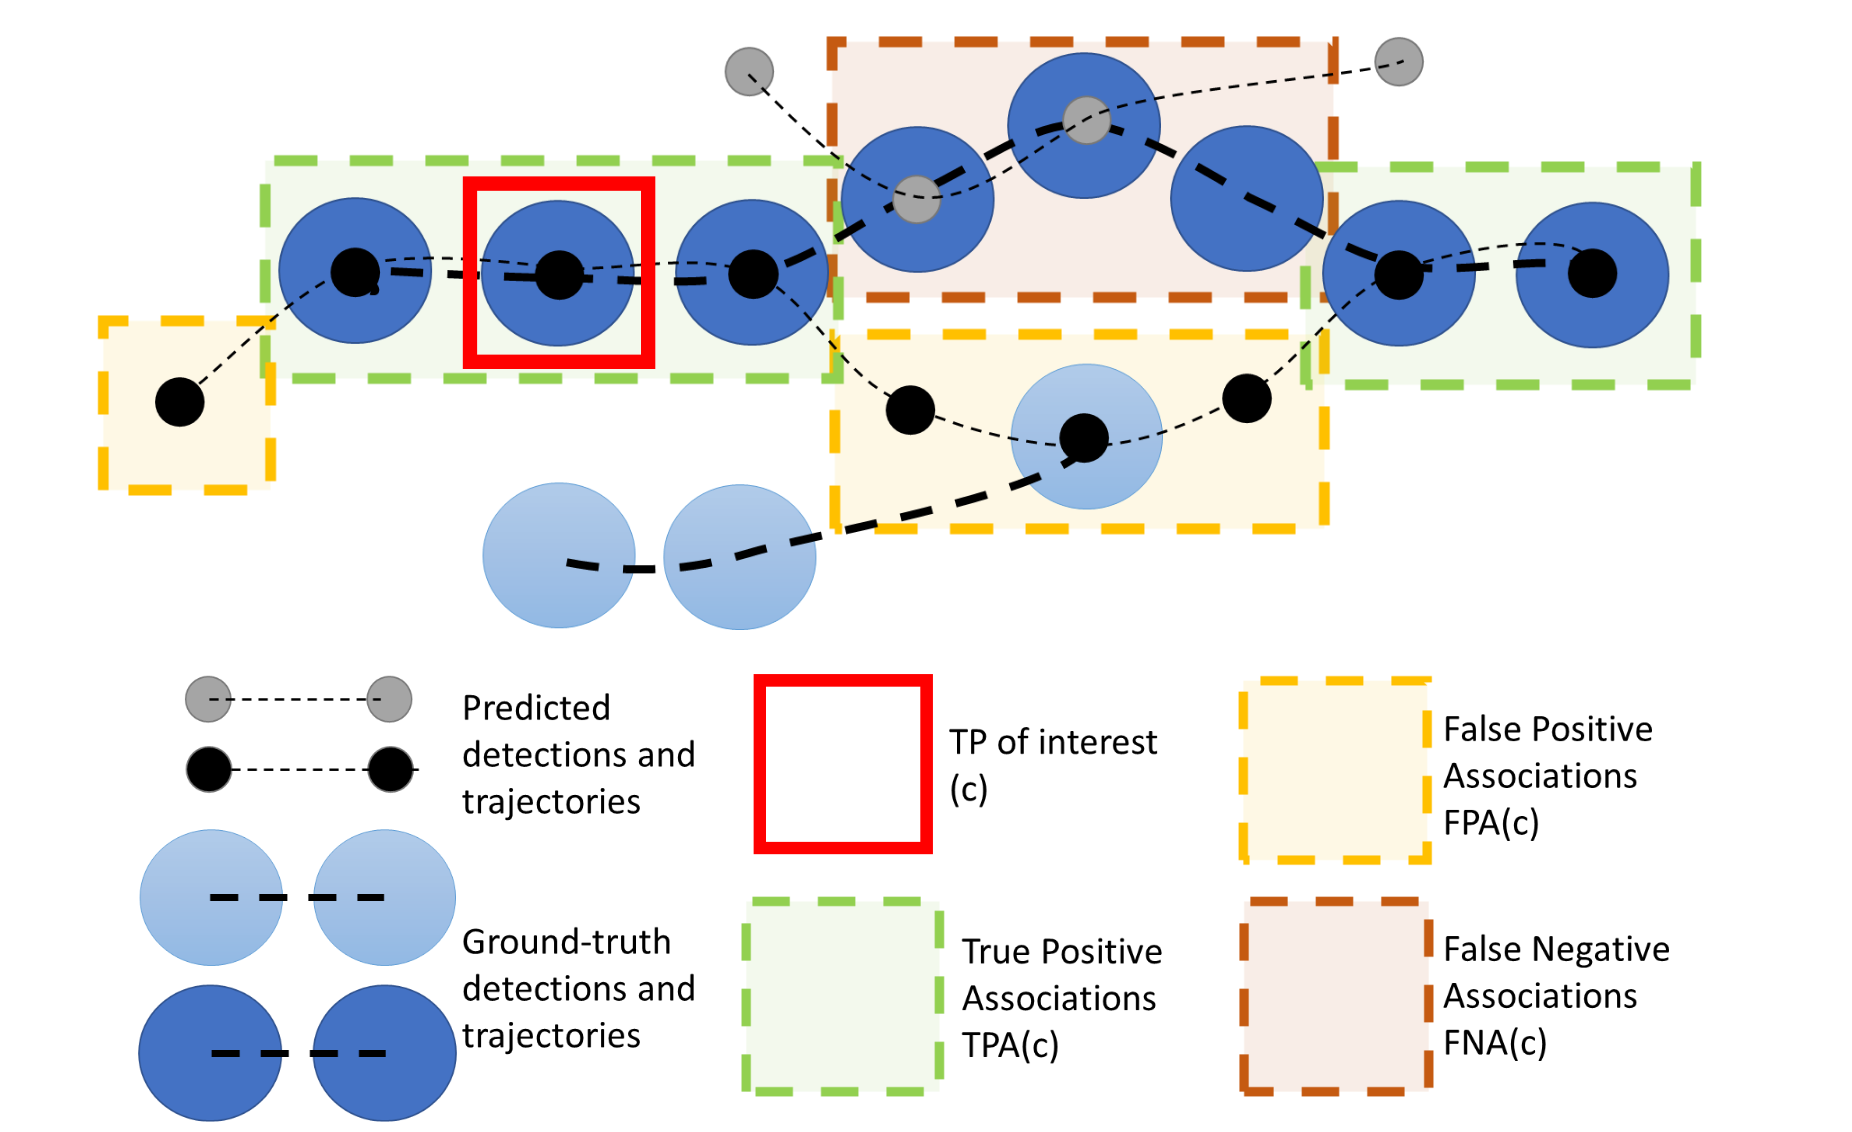
\includegraphics[width=1\textwidth]{images/T/explanation.png}
    \caption{.}
    \label{img:road}
\end{figure}

Nakoniec kompozíciou detekcie a asociácie je vypočítaná hodnota HOTA \ref{e:hota}. TODO We see that HOTA is equal to the geometric mean of a detection score and an association score. This formulation ensures that both detection and association are evenly balanced, unlike many other tracking metrics, and that the final score is somewhere between the two. It also ensures that both the detection score and association score have the same structure.
\begingroup
\large
\begin{equation}
LocA = \frac{A}{B}
\label{e:hota}
\end{equation}
\endgroup
\\
Každá sledovacia metóda bola spustená viackrát s iným nastavením. Najlepšie výsledky pre každú metódu sú zapísané v tabuľke \ref{table:hota1}. Po vyhodnotení vidno, že náš odhad najlepšej metódy sa potvrdil.
\\
\begin{table}[ht]
\centering
\begin{tabular}{|c c c c c c c c c|} 
 \hline
TODO metóda & HOTA & DetPr & DetRe & DetA & AssPr & AssRe & AssA & LocA \\ [0.5ex] 
 \hline
strongsort & 39.152 & 63.357 & 54.578 & 42.673 & 70.841 & 42.888 & 35.937 & 88.932 \\ [0.1ex]
deep & 39.152 & 63.357 & 54.578 & 42.673 & 70.841 & 42.888 & 35.937 & 88.932 \\ [0.1ex]
oc & 37.936 & 58.479 & 54.554 & 40.455 & 74.731 & 42.579 & 35.638 & 88.581 \\ [0.1ex]
byte & 27.760 & 37.434 & 34.147 & 22.085 & 57.887 & 47.258 & 34.957 & 88.027 \\ [0.1ex]
bot & 27.141 & 40.139 & 38.162 & 24.812 & 40.389 & 56.746 & 29.729 & 87.301 \\ [0.1ex]
 \hline
\end{tabular}
\caption{TODO, výsledky 4.}
\label{table:hota1}
\end{table}
\\
TODO We can see how well methods perform in each of the dimensions of detection (x-axis) and association (y-axis) separately, with the curves in the background showing how the overall HOTA score increases as both detection and association scores increase. We can go further than just comparing detection and association. Because they are both naturally decomposable into one component.
\begin{figure}[ht]
    \centering
    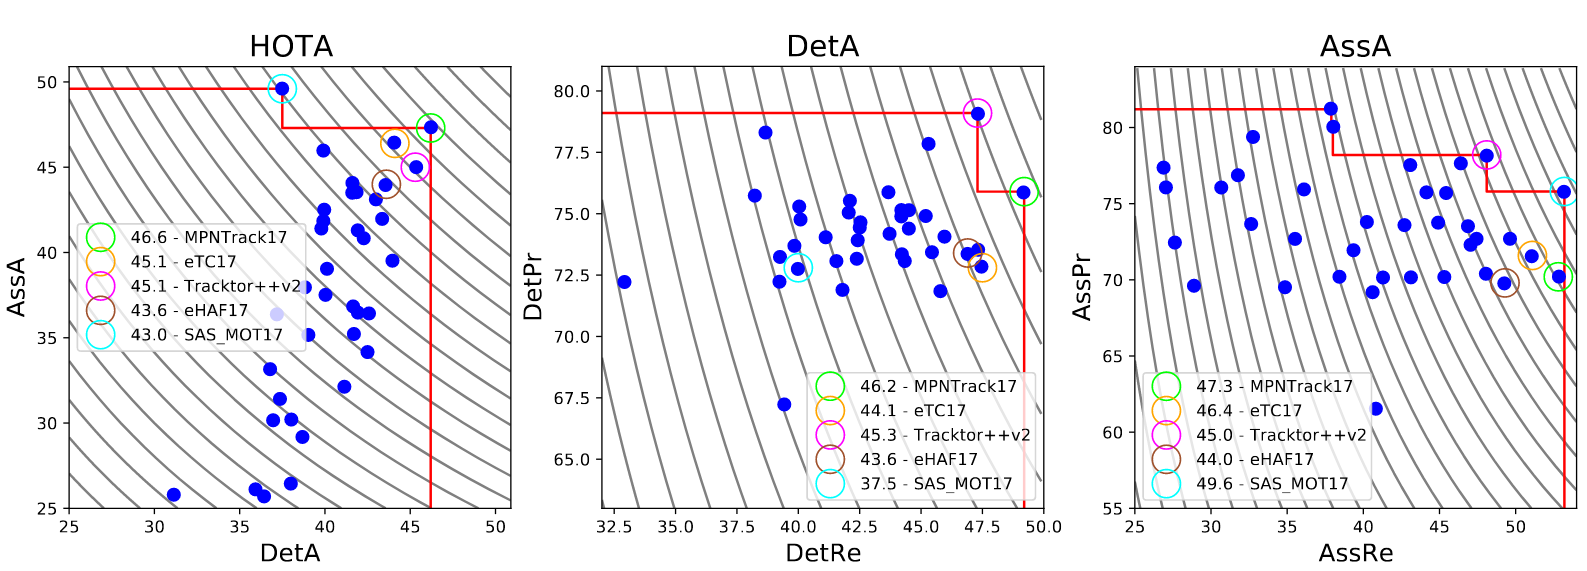
\includegraphics[width=1\textwidth]{images/T/compare.png}
    \caption{.}
    \label{img:road}
\end{figure}

TODO Tu je vizualizácia sledovania reklám z videa. Na pravej strane obrázka je metóda X a na ľavej Y. Snímky sú v tomto prípade zachytené každých 10 snímok a vidíme, že metóda Y nepriradila referenciu po oklúzii správne.
\begin{figure}[ht]
    \centering
    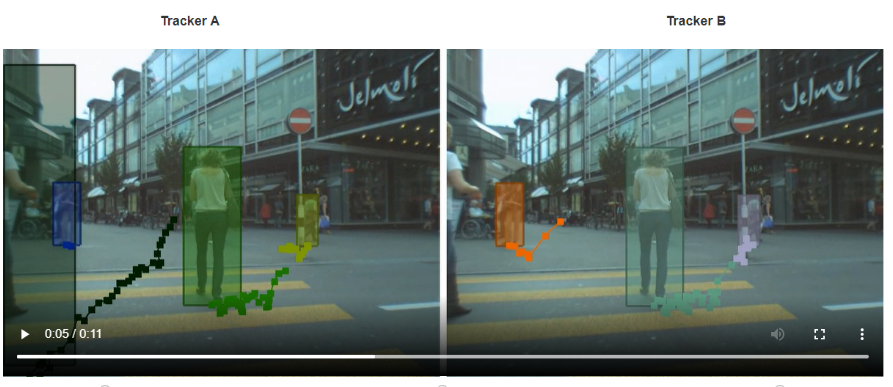
\includegraphics[width=1\textwidth]{images/T/vs.png}
    \caption{.}
    \label{img:road}
\end{figure}

To či sa vodič pozrel na reklamy sme vyhodnotili vypočítaním prieniku označenej reklamy so zaznamenanou súradnicou s polomerom 20 pixlov. Dokopy bolo na zvolenej trase nájdených 145 reklám, ktoré sa podľa počtu prienikov rozdelili do štyroch kategórií. V tabuľke \ref{table:cat} je pre každú kategóriu zapísané časové rozmedzie korešpondujúce počtu snímok s prienikom, počet reklám vyhodnotených do príslušnej kategórie a priemerný počet účastníkov, ktorý sa na reklamu danej kategórie pozreli.
% todo pridať obrázok, kde je fixácia
\\
\begin{table}[ht]
\centering
\begin{tabular}{|c c c c|}
 \hline
 kategória &	rozmedzie &	počet reklám &	počet účastníkov \\ [0.5ex] 
 \hline
slabá &	0 ms &	27 &	- \\ [0.1ex]
nízka &	1-249 ms &	66 &	2.95 \\ [0.1ex]
stredná &	250-499 ms &	18 &	5.11 \\ [0.1ex]
vysoká &	500+ ms &	3 &	2 \\ [0.1ex]
 \hline
\end{tabular}
\caption{TODO, výsledky 5.}
\label{table:cat}
\end{table}

% optimalizácia hyperparametre, Under/over-fitting
% augmentacia pred trenovanim, pri testovani (Test time augmentation)
% porovnanie precision a recall pre detector vs tracker
% porovnať chybosť kategorizácie, kebyže sa to počíta zo standardného modelu
% porovnať chybosť klasifikácie, kebyže sa to počíta zo standardného modelu

%If your use-case contains many occlussions and the motion trajectiories are not too complex, you will most certainly benefit from updating the Kalman Filter by its own predicted state. Select the number of predictions that suits your needs here: https://github.com/mikel-brostrom/Yolov5_StrongSORT_OSNet/blob/b1da64717ef50e1f60df2f1d51e1ff91d3b31ed4/trackers/strong_sort/configs/strong_sort.yaml#L7
